\pdfoutput=1
\documentclass[twocolumn]{aastex61}
%%\documentclass[]{emulateapj}

%Accepted/received/... %%

\received{xxx}
\revised{yyy}
\accepted{zzz}

%% Command to document which AAS Journal the manuscript was submitted to.
\submitjournal{AAS Journals}

%% Short title/authors

\shorttitle{Reproducing Kepler Stellar Rotation Periods}
\shortauthors{Fleming et al.}

%% Begin document, title, packages %%
\usepackage{hyperref}
\usepackage{xspace}
\usepackage{graphicx}
\usepackage{amsmath}
\usepackage[caption=false]{subfig}

%% Custom commands
\def\mearth{{\rm\,M_\oplus}}
\def\rearth{{\rm\,R_\oplus}}
\def\msun{{\rm\,M_\odot}}
\def\rsun{{\rm\,R_\odot}}
\def\lsun{{\rm\,L_\odot}}
\def\gsim{~\rlap{$>$}{\lower 1.0ex\hbox{$\sim$}}}
\def\lsim{~\rlap{$<$}{\lower 1.0ex\hbox{$\sim$}}}

\newcommand{\vplanet}[0]{\texttt{VPLANET}\xspace}
\newcommand{\eqtide}[0]{\texttt{EQTIDE}\xspace}
\newcommand{\stellar}[0]{\texttt{STELLAR}\xspace}


%% Begin doc %%

\begin{document}

\title{Reproducing Stellar Rotation Periods in the Kepler Field via Magnetic Braking and Tidal Torques}

%% AUTHORS %%

%%\correspondingauthor{David P. Fleming}
%%\email{dflemin3@uw.edu}

%%\author[0000-0001-9293-4043]{David P. Fleming}
\author{David P. Fleming}
\affil{Astronomy Department, University of Washington \\
Box 951580, Seattle, WA 98195}

\author{Rory Barnes}
\affiliation{Astronomy Department, University of Washington \\
Box 951580, Seattle, WA 98195}

\author{James R. A. Davenport}
\affiliation{Astronomy Department, University of Washington \\
Box 951580, Seattle, WA 98195}

\author{Rodrigo Luger}
\affiliation{Center for Computational Astrophysics, Flatiron Institute \\
New York, NY 10010}

%% ABSTRACT %%

\begin{abstract}

Stellar rotation period (P$_{rot}$) studies have produced numerous insights into the angular momentum evolution of low-mass stars, but previous investigations have focused on single stars even though roughly half of Sun-like stars are in stellar binaries. We examine the impact of unresolved stellar binaries on the stellar P$_{rot}$ distribution of the \textit{Kepler} field by performing Monte Carlo simulations of a population composed of single and double stars by modeling stellar evolution, magnetic braking, and tidal forces. We find that tides modify stellar rotations in all binaries with orbital periods up to 70 days.  At short orbital periods, most stellar binaries tidally-lock into synchronous rotation, naturally explaining the observed population of fast rotators in the \textit{Kepler} field that cannot be reproduced by single-star-only models.  Many binaries with longer orbital periods, some up to orbital periods of 70 days, tidally-lock, synchronizing the stellar P$_{rot}$ with the binary orbital period, causing P$_{rot}$ to not be a valid proxy for age in all cases, i.e. gyrochronology methods must be applied carefully. Our assumed flat stellar age distribution over $1-4$ Gyr underpredicts the number of fast rotators in the \textit{Kepler} field. If instead we assume a bimodal stellar age distribution in the \textit{Kepler} field composed of a young ($100$ Myr$-1$ Gyr old) and an old ($1-4$ Gyr) population, we successfully reproduce the \textit{Kepler} P$_{rot}$ distribution.

\end{abstract}

%% KEYWORDS %%

\keywords{binaries: close}

%% INTRO %%

\section{Introduction} \label{sec:intro}

Measuring stellar rotation periods via star spot modulation is a critical tool for understanding stellar angular momentum evolution in low-mass stars (M$\lsim 1.2$ M$_{\odot}$). As stars evolve, angular momentum conservation dictates that their evolving moments of inertia necessarily change their P$_{rot}$, e.g. stars spin-up as their radii contract, whereas magnetic braking, the coupling of the corotating stellar wind with the stellar magnetic field, removes angular momentum from the star, causing the observed long-term spin-down of stars \citep{Parker1958,Skumanich1972}.  

Extensive measurements of ${>}10,000$ stellar rotation periods in the \textit{Kepler} field \citep{Borucki2010,McQuillan2013,Reinhold2013,McQuillan2014,Reinhold2015,Lurie2017} have provided exquisite observational constraints for theorists to model long-term stellar angular momentum evolution. Various models have been developed to explain the observed P$_{rot}$ distribution in the \textit{Kepler} field \citep[e.g.][]{Matt2015,vanSaders2018} and to link the long-term spin-down of low-mass stars to their ages, a method known as gyrochronology \citep{Skumanich1972,Barnes2003,Barnes2007,Mamajek2008,Barnes2010}. These models, however, have failed to reproduce the large observed population of rapid rotators (P$_{rot} {\lsim} 7.5$ days) across all stellar masses in the \textit{Kepler} field \citep{McQuillan2013,McQuillan2014}.  Both gyrochonology relations \citep{McQuillan2014} and a modern magnetic braking model \citep{Matt2015} suggest that these fast rotators could be at most 1 Gyr old, in tension with the expected older ages of \textit{Kepler} field stars \citep{Chaplin2014,Angus2015}.

The aforementioned models have two limitations.  First, these models assumed stellar populations composed solely of single stars, whereas roughly half of Sun-like stars are in stellar binaries \citep{Raghavan2010,Duchene2013}. Binaries are difficult to detect in photometric surveys because of low transit probabilities, so typically they are isolated using magnitude cuts \citep[e.g.][]{Davenport2018,Simonian2018}. However, 1000s of eclipsing binaries are known in the \textit{Kepler} field \citep{Kirk2016}, with likely many more unresolved binaries present in the data. In short-period binaries, tidal torques modify stellar rotations by driving the binary towards the tidally-locked state \citep{Zahn1989,Fleming2018}. Tidal forces in binaries are commonly understood to act in binaries with orbital periods (P$_{orb}$) ${\lsim} 10$ days \citep[e.g.][]{Zahn1989,Meibom2005}, however \citet{Lurie2017} measured 100s of \textit{Kepler} eclipsing binary stellar rotation periods using starspot variability and found that tides can synchronize stellar binary rotation periods up to P$_{orb} \approx 45$ days.  Recently \citet{Simonian2018} found that most rapid rotators in the \textit{Kepler} field are likely non-eclipsing, tidally-synchronized short-period binaries. Clearly, unresolved stellar binaries impart a significant signal in P$_{rot}$ distributions, particularly in the \textit{Kepler} field at short P$_{orb}$, but can also influence P$_{rot}$ measurements at larger binary P$_{orb}$.  

Second, no previous study has simulated how a bimodal age distribution in the \textit{Kepler} field, suggested by \citet{McQuillan2014}, \citet{Matt2015}, and \citet{Davenport2017}, could explain the observed population of rapid rotators.  If the age distribution is in fact bimodal, a young, fast rotating population could explain the observed P$_{rot}$ distribution.  Here, we perform the first forward modeling of the angular momentum evolution of a realistic stellar population of single and double stars, accounting for stellar evolution, magnetic braking, tidal torques in stellar binaries, and testing the impact of a bimodal age distribution to reproduce the observed P$_{rot}$ distribution in the \textit{Kepler} field.

%Here, we examine the role of unresolved, tidally-interacting stellar binaries in the \textit{Kepler} field using a stellar evolution model, with magnetic braking, coupled with a secular equilibrium tidal model for stellar binaries. to see if their presence can explain features in the \textit{Kepler} P$_{rot}$ distribution. In $\S$~\ref{sec:methods} and $\S$~\ref{sec:simulations}, we describe our computational methods and simulation set-up, and discuss our results and their implications in $\S$~\ref{sec:results} and $\S$~\ref{sec:discussion}, respectively.

%% Maybe just focus on Kepler Prot observations?
% in clusters \citep[e.g. Praesepe;][]{Scholz2007,Scholz2011,Agueros2011,Delorme2011,Kovacs2014,Douglas2017} and extensive P$_{rot}$ measurements
 
%% SECTION : Methods %%

\section{Methods} \label{sec:methods}

\subsection{Stellar Evolution} \label{sec:methods:stellar}

We simulate stellar rotation evolution for both single stars and stellar binaries using the coupled stellar-tidal evolution model presented in \citet{Fleming2018} and implemented in the open-source code VPLanet\footnote{VPLanet is publically available
at \href{https://github.com/VirtualPlanetaryLaboratory/vplanet}{{https://github.com/VirtualPlanetaryLaboratory/vplanet}}.} \citep[][Barnes et al., in prep]{Barnes2016}. We improve upon the stellar evolution model used in \citet{Fleming2018}, \stellar, by tracking the evolution of both the stellar radius of gyration, $r_g$, and radius, using a bicubic interpolation over mass and time of the \citet{Baraffe2015} stellar evolution models. We model stellar spin-down due to magnetic braking using the model derived in \citet{Matt2015} since it has been shown to successfully reproduce many features in the P$_{rot}$ distribution of the \textit{Kepler} field, notably the upper and lower envelopes of the latter distribution and the observed ``dip" in the distribution around M${\approx}0.6$ M$_{\odot}$. We integrate the following equation to model the net change in the stellar rotation rate due to stellar evolution and magnetic braking: 

\begin{equation} \label{eqn:stellar_rot_rate_dt}
\dot{\omega} = \frac{\dot{J}_{mb}}{I} - \frac{2 \dot{R} \omega}{R} - \frac{2 \dot{r_g} \omega}{r_g}
\end{equation}
where the moment of inertia $I = M r_g^2 R^2$ and $\dot{J}_{mb}$ is the angular momentum loss due to magnetic braking.  

\subsection{Tidal Evolution} \label{sec:methods:eqtide}

For stellar binaries, we assume that they tidally interact via the ``Constant Phase Lag" (CPL) version \citep[][]{FerrazMello2008,Heller2011} of the commonly used equilibrium tidal model \citep{Darwin1880}.  The CPL model tracks the secular evolution of the binary's semi-major axis, $a$, eccentricity, $e$, and stellar rotation rates, $\omega$, due to tidal torques.  The CPL model assumes that the tidal torque on one star due to its companion arises from a linear combination of uncoupled tidal bulges, each with their own associated frequency, that maintain a fixed phase with respect to the line connecting the two stars' centers of mass and is analogous to a driven, damped harmonic oscillator \citep{Greenberg2009}. We use the \eqtide implementation of the CPL model in VPLanet described in \citet{Fleming2018}, their equations 8-16, and simultaneously integrate those equations with Eq.~(\ref{eqn:stellar_rot_rate_dt}) for stellar binaries.  All equations are integrated using a $4^{th}$ order Runge-Kutta scheme.

%Following \citet{Fleming2018}, when one or both binary stars are tidally locked, we assume that tidal forces prevent magnetic braking from spinning down the tidally locked star(s), but instead, any angular momentum lost is lost at the expense of the binary orbit, decreasing the orbital semi-major axis as a result.  Below in Eq.~(\ref{eqn:tidal_locked_one}) and Eq.~(\ref{eqn:tidal_locked_two}), we modify Eqs. (18) and (20) from \citet{Fleming2018} to account for $r_g$ evolution for the cases when one or both stars tidally lock under conservation of angular momentum, respectively:
%\small
%\begin{equation} \label{eqn:tidal_locked_one}
%\begin{split}
%\dot{a}_{coupled}^{(1)} = \frac{-\dot{J_{mb}} - 2 \omega \left( m_1 r_{g,1}^2 R_1 \dot{R_1} - m_1 r_{g,1} \dot{r}_{g,1} R_1^2 \right)}
%{\frac{\mu^2 G M (1-e^2)}{2J_{orb}} - \frac{3 \omega}{2a} m_1 r_{g,1}^2 R_1^2}
%\end{split}
%\end{equation}
%\normalsize
% and
% \small
%\begin{equation} \label{eqn:tidal_locked_two}
%\begin{split}
%\dot{a}_{coupled}^{(2)} = \frac{-\dot{J_{mb}} - 2 \omega \left( \sum_{i=1}^{2} m_i r_{g,i}^2 R_i \dot{R_i} + m_i r_{g,i} \dot{r}_{g,i} R_i^2 \right)}
%{\frac{\mu^2 G M (1-e^2)}{2J_{orb}} - \frac{3 \omega}{2a} \left( m_1 r_{g,1}^2 R_1^2 + m_2 r_{g,2}^2 R_2^2 \right)}
%\end{split}
%\end{equation}
%\normalsize
%where $J_{orb}$ is the orbital angular momentum.

%% SECTION: Simulations + Initial conditions %%

\subsection{Simulations} \label{sec:simulations}

We simulate the P$_{rot}$ distribution of the \textit{Kepler} field by performing Monte Carlo study consisting of a population of 10,000 stellar systems composed of single stars and binaries using VPLanet. For each simulation, we sample the stellar mass from a Gaussian fit to the stellar mass distribution in \citet{McQuillan2014} with $\mu=0.885$ M$_{\odot}$ and $\sigma=0.201$ M$_{\odot}$ to approximate the \textit{Kepler} mission's intended selection bias of monitoring FGK stars for Earth-like planets. We restrict stellar masses to be within [$0.1,1.2$] M$_{\odot}$ to limit the influence of subgiants since more massive stars evolve off the main sequence after $\gsim 4$ Gyr, our age limit, and because more massive stars do not experience magnetic braking due to their shallow convective envelopes \citep{Kraft1967}. Following \citet{Matt2015}, we uniformly sample the log$_{10}$ of P$_{rot}$ over [$0.8,15$] days, a distribution that approximates the P$_{rot}$ distribution of stars in the ${\sim}2$ Myr old ONC.  We randomly assign stars a stellar companion according to stellar multiplicity fractions from \citet{Duchene2013}. In binaries, we compute the secondary star's mass by uniformly sampling the mass ratio over [$0.1, 1$] following observations of mass ratios in low-mass binaries \citep{Raghavan2010}.We uniformly randomly sampling the initial eccentricity ($e$) over [$0.0,0.3$] and stellar tidal Qs are sampled from a log-uniform distribution over $[10^5,10^8]$. For the initial binary $P_{orb}$, we test two models. In Model 1, $10\%$ of binaries have their initial P$_{orb}$ uniformly sampled over [$3,80$] days, consistent with P$_{orb}$ distributions of field stars \citep[e.g.][]{Raghavan2010}, and the remaining $90\%$ have P$_{orb} > 80$ d and are considered ``single" stars since for P$_{orb} > 80$ d, tidal torques are sufficiently weak such that the stars' evolution is effectively independent of their companion.  In Model 2, we consider an enhanced population of short period binaries by sampling all initial P$_{orb}$ uniformly over [$3,80$] days.  

In Models 1 and 2, we simulate each system to an age uniformly sampled over [$1,4$] Gyr, the approximate age range of \textit{Kepler} field stars \citep{McQuillan2014,Angus2015}, with the upper-limit suggested by \citet{McQuillan2014} and \citet{Matt2015}. We also consider a ``Two Population" model that uses the initial conditions of Model 2 and assumes that $40\%$ of stars comprise a ``young" population with ages uniformly sampled over [$0.1,1$] Gyr, while the remainder comprise the ``old" population with ages uniformly sampled over [$1,4$] Gyr. We track the P$_{rot}$ evolution for each single star and the primary, i.e. more massive star, in binaries as it is observationally easier to measure a P$_{rot}$ due to starspot modulations on the more massive, and hence brighter, star. We compare our simulation results with the \textit{Kepler} P$_{rot}$ distribution measured by \citet{McQuillan2014}.

All code used to run simulations and generate figures is available online\footnote{\href{https://github.com/dflemin3/binGyro}{https://github.com/dflemin3/binGyro}.} with accompanying descriptions and documentation.

%  For simulations of binaries, given the inherent uncertainty in and complexity of the formation of binaries \citep[e.g.][]{Bonnell1994,Bate2000,Bate2002,Moe2018} and the potential for dynamical processing via tides or stellar close encounters \citep[e.g.][]{Mardling2001,Hurley2002,Ivanova2005,Meibom2005}, we take an agnostic approach to the initial orbital configuration. 

%Our goal is to determine how the distribution of $P_{rot}$ for a population stars composed solely of single stars differs, if at all, from a population of both single stars and binaries.  If there is a substantial difference between the two distributions, e.g. tidally-locked fast rotators, then any study examining the distribution of stellar $P_{rot}$ should therefore account for the impact of tidally-interacting stellar binaries.  We approach this problem with a ...

%% SECTION: VPLANET RESULTS %%

\section{Results} \label{sec:results}

\subsection{Tidal Locking in Stellar Binaries} \label{sec:results:locking}

Here we examine the tidal locking in binaries using the simulations from Model 2 (see $\S$~\ref{sec:results:kepler2}) by plotting P$_{rot}$ as a function of mass and age for binaries in Fig.~\ref{fig:locking}. We find that $35.5\%$ of binaries tidally lock before the age of the system, typically for tidal $Q \lsim 10^7$. Tidally-locked binaries tend to rotate more rapidly than unlocked binaries, reflected in the increased density for P$_{rot} \lsim 20$ d in the marginal distribution for the locked population and in the distribution medians (locked median P$_{rot} = 19.8$ d compared to unlocked median P$_{rot} = 27.5$ d). Binaries readily tidally-lock at short P$_{orb}$ due to the tidal force's strong semi-major axis dependence, increasing the strength of tidal torques at shorter orbital separations. When stellar binaries approach the tidally-locked state, tidal torques overpower the torque due to magnetic braking, fixing P$_{rot} = $P$_{orb}$, resulting in long-lasting rapid rotation in short P$_{orb}$ binaries. 

Tidal forces modify the spins of unlocked binaries as well, tending to spin-up stars against the effects of magnetic braking towards orbital synchronization, reflected in unlocked binaries' median P$_{rot} = 27.5$ d, compared to the single star median P$_{rot} = 30.6$ d. Tidal locking is not limited to P$_{orb} \lsim 10$ d, however, as we observe stellar binaries to tidally lock out up to P$_{orb} \approx 70$ d, producing a slow-rotating population above the P$_{rot}$ distribution envelop of single stars (compare to Fig.~\ref{fig:kepler2}). This behavior is consistent with observations of P$_{rot}$ in \textit{Kepler} eclipsing binaries by \citet{Lurie2017} who find that binaries can tidally lock up to their detection limit of P$_{orb} = $ P$_{rot} = 45$ d. The observed age distribution of tidally-locked binaries has little dependence on P$_{rot}$, with both young and old systems tidally-locking at long and short P$_{rot}$, causing the predictions of gyrochronology models to fail in such systems. 

\begin{figure}[h]
	\includegraphics[width=0.45\textwidth]{../Plots/locked_kepler.pdf}
   \caption{Simulated distribution of P$_{rot}$ for tidally-locked (cross) and unlocked (circle) stellar binaries, colored by age for Model 2 (see $\S$~\ref{sec:results:kepler2}). Left: P$_{rot}$ as a function of stellar mass.  Right: Marginalized P$_{rot}$ distribution for locked (blue) and unlocked (orange) binaries.  Tidally-locked binaries rotate more rapidly than unlocked binaries, displaying an increased density in the P$_{rot}$ distribution for P$_{rot} {\lsim} 20$ d, and with a median P$_{rot} = 19.8$ d, compared to the unlocked median P$_{rot} = 27.5$ d. Unlocked binaries on average rotate more quickly than single stars (compare to single distribution in Fig.~\ref{fig:kepler2}) due to the influence of tidal torques.}
    \label{fig:locking}
\end{figure}

\subsection{Comparison to \textit{Kepler}}

\subsubsection{Model 1} \label{sec:results:kepler1}

In Fig.~\ref{fig:kepler1}, we display our simulated P$_{rot}$ for Model 1, compared to the observed \textit{Kepler} distribution \citep{McQuillan2014}. Single stars, defined as stars without a companion, or with a companion with a P$_{orb} > 80$ d where tides do not modify the orbit or stellar rotations, rotate more slowly with age due to magnetic braking, with more massive stars rotating more quickly than low mass stars, consistent with \textit{Kepler} P$_{rot}$ observations.  There is a larger spread in P$_{rot}$ for stars with M$\lsim 1$ M$_{\odot}$ with the spread increasing with decreasing stellar mass, due to the mass-dependence magnetic braking torque in the \citet{Matt2015} model.
%in which lower mass stars tend to spin down more quickly than higher-mass stars once they enter the "unsaturated" regime (see \citet{Matt2015} equations 6 and 7).

The inclusion stellar binaries naturally produces a population of fast rotators (P$_{rot} < 7.5$ d) across all masses as binaries readily tidally-lock at shorter P$_{orb}$, with ${\sim}90\%$ of stars in this P$_{rot}$ regime being tidally-locked binaries. Single-star only models fail to reproduce this feature.  The fast rotator population only comprises $0.25\%$ of all simulated stars, compared to $16\%$ of \textit{Kepler} stars in the same regime, and is therefore insufficient to explain the observed population of fast rotators. Our simulated P$_{rot}$ distribution is systematically biased towards longer P$_{rot}$ than the \textit{Kepler} distribution with a total median P$_{rot} = 30.3$ d compared to \textit{Kepler} median P$_{rot} = 17.3$ d. The inclusion of binaries does little to shift the P$_{rot}$ distribution towards shorter P$_{rot}$ as Model 1's assumed binary P$_{orb}$ distribution, based on observations of field stars \citep{Raghavan2010}, predicts that only ${\sim}4\%$ of all stars will be in stellar binaries with P$_{orb} < 80$ d, short enough for tides to appreciably modify stellar rotations. 

\begin{figure*}[ht]
	\includegraphics[width=\textwidth]{../Plots/kepler_box_dist_corr.pdf}
   \caption{Simulated distribution of P$_{rot}$ for single (circle) and double (cross, defined as stellar binaries with P$_{orb} < 80$ d) stars for Model 1. Left: P$_{rot}$ as a function of stellar mass, colored by age.  Center: Marginalized P$_{rot}$ distributions for single stars (orange), binary stars (green), and the total sample (blue), and \textit{Kepler} \citep{McQuillan2014} (red). Except for a few low-mass (${\lsim}0.3$M$_{\odot}$) single stars, regardless of age, rotate more slowly (single median P$_{rot} = 30.5$ d) than \textit{Kepler} stars (\textit{Kepler} median P$_{rot} = 17.3$ d) and fail to explain the observed population of fast rotators.  Binaries, however, readily tidally-lock at shorter P$_{orb}$, naturally producing a population of fast rotators (binary median P$_{rot} = 25.9$ d). Right: box-and-whisker plot of the P$_{rot}$ distribution for the simulations seen in the left panel in 0.1 M$_{\odot}$ bins. The shaded regions cover the distributions' interquartile range, the white lines indicate the medians, and the whiskers do not indicate error bars, but rather the spread of the distribution, extending to the 5th and 95th percentiles. The numbers over the boxes indicate the percent difference between the single (orange) and total (blue) distribution medians with the \citet{McQuillan2014} (red) sample. Even with the inclusion of binaries that tidally-lock at short P$_{rot}$, Model 1 produces a more slowly rotating stellar population than is observed in the \textit{Kepler} field, indicating that our assumed stellar population is incorrect.}%
    \label{fig:kepler1}%
\end{figure*}

\subsubsection{Model 2: Enhanced Binary Population} \label{sec:results:kepler2}

In Model 2, we attempt to increase the number of fast rotators by increasing the number of systems that could tidally-lock at short P$_{rot}$.  We assume all stellar binaries have a P$_{orb}$ uniformly sampled over [$3,80$] d, as opposed to just $10\%$ of binaries in Model 1.  Although optimistic, our assumption is reasonable as an analysis of fast rotators in the \textit{Kepler} field by \citet{Simonian2018} found that $\sim 59\%$ of stars with $1.5 <$ P$_{rot} < 7$ d are likely unresolved, tidally-locked binaries, suggesting that a substantial short-period rapidly rotating binary population does exist in the \textit{Kepler} field.

As in Model 1, stellar binaries tidally-lock at short P$_{rot}$ producing a population of fast rotators below the single star sequence with binaries comprising ${\sim}99\%$ of fast rotators.  The inclusion of additional short P$_{orb}$ binaries noticeably modifies the simulated P$_{rot}$ distribution, shifting the median P$_{rot}$ for the total sample down to $28.6$ d, compared to $30.6$ d for the single-star-only distribution.  The impact of binaries is evident across all masses in the right panel of Fig.~\ref{fig:kepler2} as the total P$_{rot}$ distribution, which includes binaries, better matches the observed \textit{Kepler} distribution than the single star only distribution, due to the fast rotating tidally-locked binary population.  The enhanced binary population of Model 2 still predicts a more slowly rotating stellar P$_{rot}$ distribution that is observed, specifically in the fast rotator regime, with Model 2 predicting $3.4\%$ of our simulated stars are fast rotators, compared to $16\%$ of \textit{Kepler} stars. As noted in $\S$~\ref{sec:results:locking}, tidally-locked binaries fix P$_{rot} = $ P$_{orb}$ as tidal torques overpower the torque due to magnetic braking, causing P$_{rot}$ in binaries to not correlate with age.

\begin{figure*}[ht]
	\includegraphics[width=\textwidth]{../Plots/kepler_box_dist.pdf}
   \caption{Identical format to Fig.~\ref{fig:kepler1}, but displaying simulated data from Model 2 (see $\S$~\ref{sec:results:kepler2}). Left: Single stars, regardless of age, rotate too slowly (single median P$_{rot} = 30.6$ d) to explain the population of fast rotators in the \textit{Kepler} field (\textit{Kepler} median P$_{rot} = 17.3$ d).  The enhanced population of short P$_{orb}$ binaries, however, naturally produces a significant population of tidally-locked binaries at P$_{rot} \lsim 20$ d (binary median P$_{rot} = 25.4$ d) that is reflected in the observed total P$_{rot}$ distribution (total median P$_{rot} = 28.6$ d). Right: For most masses, the total distribution, which includes binaries, can better reproduce the \textit{Kepler} medians and fast rotator population compared to the single-star only distribution.  Even with the addition of a large population of short-period binaries, Model 2 still underpredicts the number of fast rotators across all stellar masses.}%
    \label{fig:kepler2}%
\end{figure*}

\subsubsection{Two Population Model} \label{sec:results:kepler_two_pop}

Observations \citep{McQuillan2014,Davenport2017} and theoretical work \citep{Matt2015} suggest that the \textit{Kepler} field contains a substantial population of young stars with ages $< 1$ Gyr.  Given the inability of Models 1 and 2 to reproduce the \textit{Kepler} P$_{rot}$ distribution, especially at short P$_{rot}$, we test the hypothesize of a bimodal \textit{Kepler} stellar age distribution. We use the enhanced binary population of Model 2 and assume that $40\%$ of stars comprise the ``young" population, with ages uniformly sampled over [$0.1,1$] Gyr, while the remainder comprise the ``old" population, with ages uniformly sampled over [$1,4$] Gyr.  We display the results of these simulations in Fig.~\ref{fig:kepler_two_pop}.

We find that the inclusion of the young population substantially improves our simulated P$_{rot}$ distribution's fit to the \textit{Kepler} distribution with the total median P$_{rot} = 19.6$ d, a close match to the median P$_{rot} = 17.3$ d in the \textit{Kepler} field. In the right panel of Fig.~\ref{fig:kepler_two_pop} for $ 0.4 \textrm{M}_{\odot} \lsim \textrm{M} \lsim 1.2 \textrm{M}_{\odot}$, the inclusion of both a young population and tidally-interacting binaries in the total (blue) sample leads to an excellent match with the \textit{Kepler} distribution (red) compared to the single-star only (orange) model, emphasizing the importance of including stellar binaries in P$_{rot}$ forward models. The combination of a fast-rotating young stellar population and enhanced binary population produces a population of fast rotators (P$_{rot} < 7.5$ d) comprising $15.5\%$ of simulated stellar systems, remarkably similar to the \textit{Kepler} field's value of $16\%$.  Moreover, we find that $52\%$ of fast rotators are in stellar binaries, in excellent agreement with the suggested value of $59\%$ for likely \textit{Kepler} photometric binaries estimated by \citet{Simonian2018}.  Our simulations suggest that not only is there likely a substantial population of young stars in the \textit{Kepler} field comprising $\sim 40\%$ of all stars, but also that a substantial fractions of fast rotators in the \textit{Kepler} field are tidally-interacting binaries. Our simulations still predict a more slowly-rotating population that what is observed, suggesting that our simple bimodal age distribution should take on a different form, e.g. two Gaussians, or that stellar angular momentum evolution might proceed differently for older stars as proposed by \citet[e.g.][]{vanSaders2016,vanSaders2018}.

\begin{figure*}[ht]
	\includegraphics[width=\textwidth]{../Plots/kepler_two_pop_box_dist.pdf}
   \caption{Identical format to Fig.~\ref{fig:kepler1}, but displaying simulated data from our two population model (see $\S$~\ref{sec:results:kepler_two_pop}). Our two population model reproduces the observed \textit{Kepler} P$_{rot}$ distribution, especially the fast rotator population, with a total median P$_{rot} = 19.6$ d compared to the \textit{Kepler} median P$_{rot} = 17.3$ d, a close match. In the right panel for $ 0.4 \textrm{M}_{\odot} \lsim \textrm{M} \lsim 1.2 \textrm{M}_{\odot}$, the inclusion of tidally-interacting binaries in the total (blue) sample leads to an excellent match with the \textit{Kepler} distribution (red) compared to the single-star only (orange) model, emphasizing the importance of including stellar binaries in P$_{rot}$ forward models.}%
    \label{fig:kepler_two_pop}%
\end{figure*}

%% Old stuff %%

% Stellar evolution figure caption
% Stellar evolution for 1 M$_{\odot}$ (blue), 0.7 M$_{\odot}$, (orange), and 0.2 M$_{\odot}$ (green) stars according to our interpolation of the \citet{Baraffe2015} stellar models, magnetic braking, and assuming conservation of angular momentum according to \stellar.  We display the radius (left panel), $r_g$ (middle panel), and rotation rate (right panel) evolution for each star using two magnetic braking models from \citet{Reiners2012} (solid curve) and \citet{Repetto2014} (dashed curve).  The dot on each curve denotes the approximate time that each star reaches the main sequence.  At early times, radius contract and $r_g$ decreasing spins up the stars, while at late times, magnetic braking efficiently spins down stars.

%\begin{figure*}[ht]
%	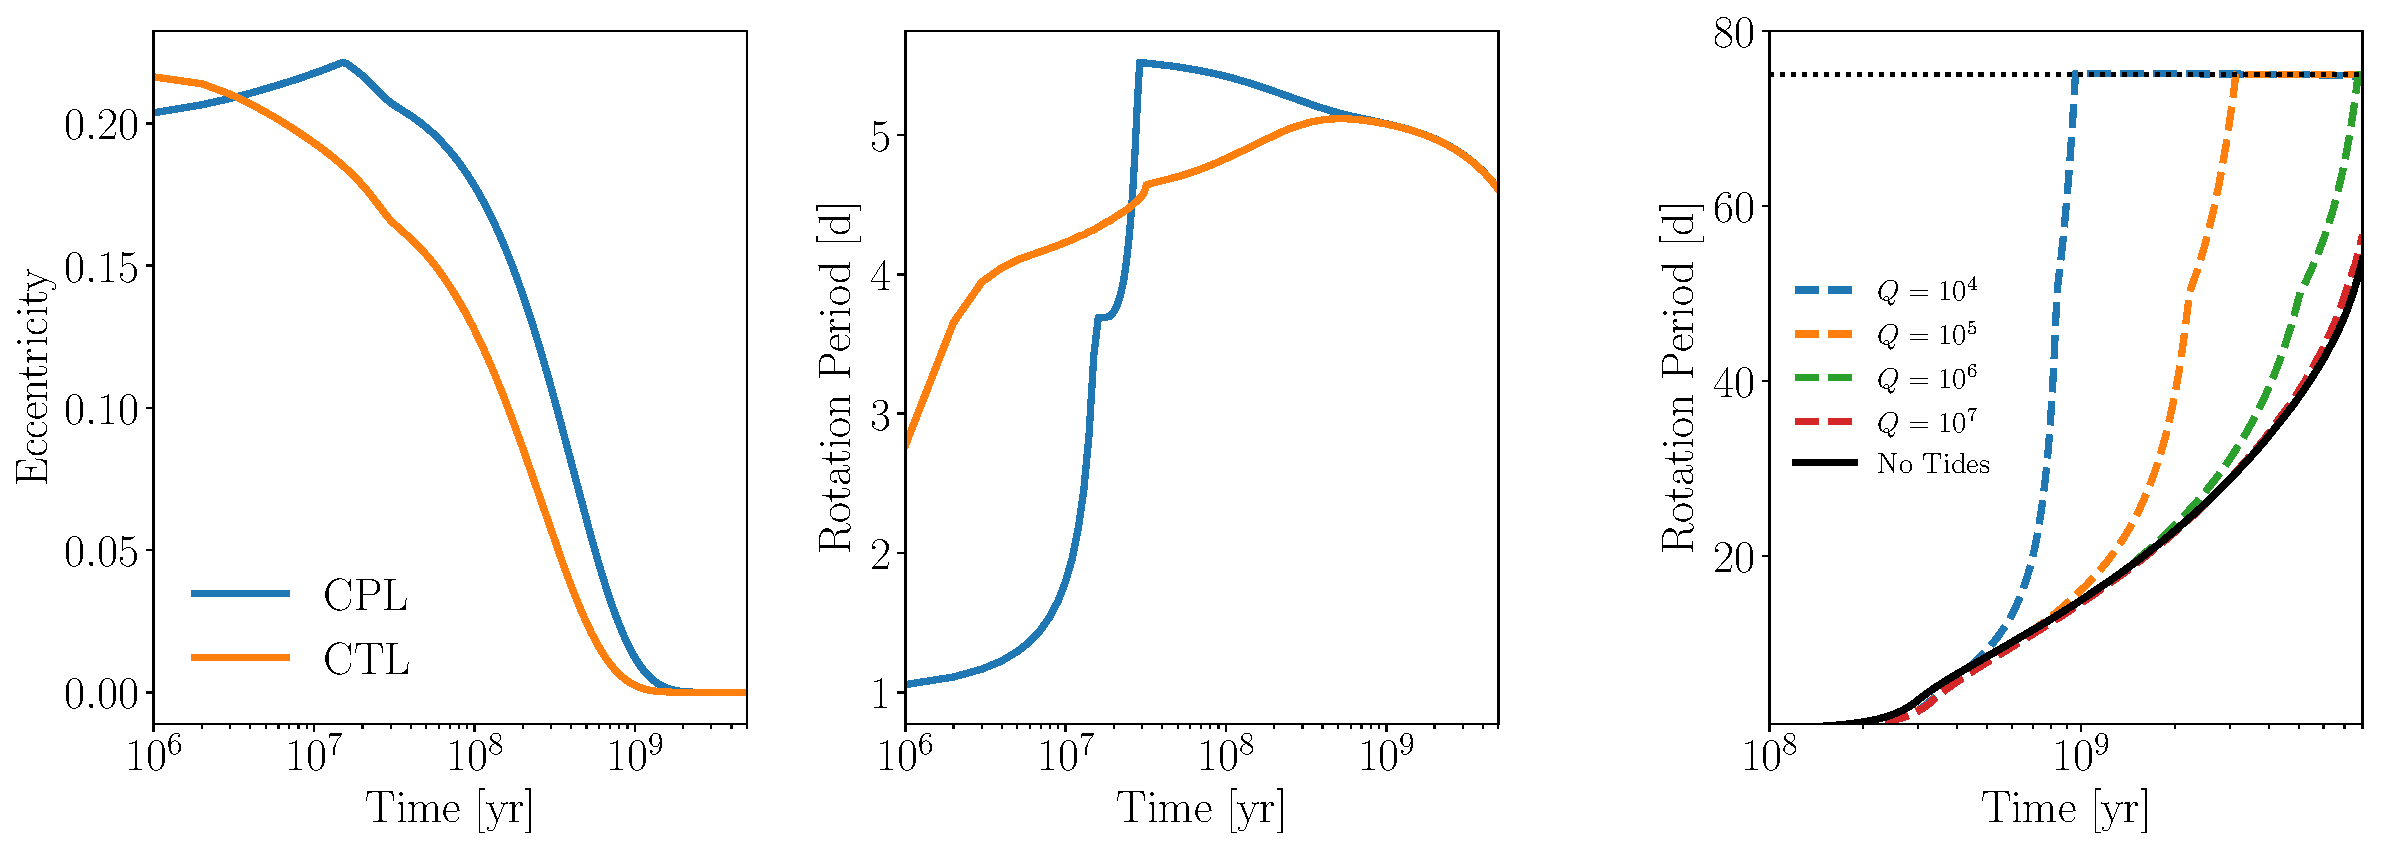
\includegraphics[width=\textwidth]{../Plots/Qrot.pdf}
%   \caption{Rotation period as a function of time for a solar mass star (No Tides, black dot-dashed curve) and solar twin binaries with initial orbital periods of 20 days (solid curves) and 50 days (dashed curves).  The dotted lines indicate rotation periods of 20 and 50 days, respectively.  The different colors of the binaries' curves denote the assumed tidal Qs, which range from $10^4$ to $10^7$.  For the first ${\sim}5 \times 10^7$ years, stellar radius contraction and $r_g$ evolution on the pre-main sequence spin up the stars.  Once the stars reach the main sequence, magnetic braking, and tides in the binary systems, slow the rotation rates.  In the long term, stellar rotation rates in binaries with lower tidal Qs slow more rapidly, and eventually all binary stars tidally lock into synchronous rotation, whereas the single star in the No Tides continues to spin down under the influence of magnetic braking.  Once the stellar binaries tidally lock, their spins undergo little evolution, with most slightly speeding up as binary orbital decay, caused by magnetic braking, slowly decreases their orbital periods.}
%    \label{fig:Qrot}
%\end{figure*}

%\subsection{P$_{rot}$ Distribution Over Time} \label{sec:results:prot_ages}

% XXX put stats discussion in results, reference them here to shorten caption
%\begin{figure}[h]
%	\includegraphics[width=0.4\textwidth]{../Plots/kepler_prot_dist_ensemble.pdf}
%  \caption{Simulated P$_{rot}$ distributions for synthetic clusters ages of 100, 300, 600 Myr, 1 Gyr, and the final age of each system, 1-4 Gyr.  For each cluster age, we gauge the impact of binarity on the P$_{rot}$ distribution by performing the two-sample Kolmogorov–Smirnov test, testing the null hypothesis that the total (blue) and single (orange) sample are drawn from the same parent distribution for a significane level $\alpha = 0.005$, or an effective $\alpha = 0.001$ after applying the Bonferroni correction \citep{Dunn1961} for testing multiple hypotheses. At 100 Myr, many stars in the sample are still contracting on the pre-main sequence, and hence the P$_{rot}$ distributions are shifted towards faster P$_{rot}$ compared to the initial distribution (black). As the stars age, the P$_{rot}$ distributions shift towards slower P$_{rot}$ due to magnetic braking.  For clusters older than 600 Myr, we can reject the null hypothesis that the single and total distributions are drawn from the same parent distribution, suggesting that the inclusion of binaries modifies the observed P$_{rot}$ distribution. This feature can be seen in the 1 Gyr old cluster as an enhancement of fast rotating stellar binaries, a signature of tidal-locking. For older field stars, the simulated distributions the impact of binaries is significant, reflected by a population of fast rotators not seen in the single population, and causes the total distribution to better reflect the \textit{Kepler} distribution.}
%    \label{fig:kepler_dist_ensemble}
%\end{figure}

%% SECTION: DISCUSSION %%

\section{Discussion} \label{sec:discussion}

For the first time, we model the angular momentum evolution of a realistic population of single and double stars, accounting for stellar evolution, magnetic braking, and tidal evolution in binaries, in order to reproduce the P$_{rot}$ distribution of \textit{Kepler} field stars.  We show that tidal forces drive stellar binaries to the tidally-locked state, naturally produce a population of fast rotators that single star models fail to produce.  We find that binaries can tidally-lock up to $P_{orb} \approx 70$ d, causing P$_{rot}$ in binaries to not be a valid proxy for age.  We show that reproducing the \textit{Kepler} P$_{rot}$ distribution requires an enhanced number of short-period binaries that comprise most of the fast rotating population, consistent with the findings of \citet{Simonian2018}, and a bimodal age distribution for \textit{Kepler} field stars, with $\approx 40\%$ of stars having ages between 100 Myr and 1 Gyr, as suggested by observations \citep{McQuillan2014,Davenport2017} and theory \citep{Matt2015}. The hypothesis of an age bimodality in the \textit{Kepler} field can be tested by measuring astroseimic ages \citep[e.g.][]{Ulrich1986,Silva2015}, for example, but also requires modeling tidal torques in binaries as P$_{rot}$ measured for unresolved, tidally-locked binaries does not correlate with age, complicating inference.

On-going observations by the extended Kepler mission \citep[K2,][]{Howell2014}, the Transiting Exoplanet Survey Satellite \citep{Ricker2014}, and Gaia \citep{Gaia2016,Lanzafame2018} will significantly increase the number of P$_{rot}$ observation for low-mass stars, providing an excellent test for models of stellar angular momentum evolution in both the field and in clusters.  We emphasize that modelling these stellar populations requires modeling tidally-interacting binaries, especially for fast rotators.

%% ACKNOWLEDGEMENTS %%
\acknowledgments
This work was facilitated though the use of advanced computational, storage, and networking infrastructure provided by the Hyak supercomputer system and funded by the STF at the University of Washington. This work was supported by NASA Headquarters under the NASA Earth and Space Science Fellowship Program - Grant 80NSSC17K0482.  DPF and RB acknowledge that this work was supported by the NASA Astrobiology Institute's Virtual Planetary Laboratory under Cooperative Agreement number NNA13AA93A. 

%% SOFTWARE %%
%\software{matplotlib: \citet{Hunter2007}, numpy: \citet{vanderWalt2011}, pandas: \citet{Mckinney2010}}

%% BIBLIOGRAPHY %%
\bibliography{binGyro}

\end{document}

%% End document %%
